\documentclass{finalReport}
% Packages
\usepackage{cleveref}
\Crefname{figure}{Fig.}{Figs.}
\crefname{figure}{Figure.}{Figures.}
\newcommand\crefrangeconjunction{--}
\newcommand\crefpairconjunction{ 그리고 }
\usepackage{subcaption}
\usepackage{graphicx}
\usepackage{lipsum}
% Theorem-like environments
\newtheorem{remark}{Remark}
\newtheorem{assumption}{Assumption}

\title{재난현장 무선통신 추적기반 요구조자 및 소방관 위치정보시스템 개발과제} % 과제명
\subtitle{이동궤적 보정 연구} % 세부과제명
\authorFirst{김 유 단} 	% 연구책임자
\authorSecond{박 찬 국}	% 참여연구원
\authorThird{이 수 원}
\authorFourth{}
\authorFirstTitle{교수}
\authorSecondTitle{교수}
\authorThirdTitle{박사과정}
\authorFourthTitle{}
\yearmonth{2021. 01} 	% 연월
\reportname{최종보고서}    % 보고서명
\begin{document}
% Title page
\maketitle
% 목차
\pagestyle{empty}
\tableofcontents
\listoffigures
\listoftables
\clearpage
\setcounter{page}{1}
\pagestyle{plain}
% 본문 시작
\section{서 론}
\subsection{연구개요}
\lipsum[1]
% Figure example
\begin{figure}[h]
	\centering
	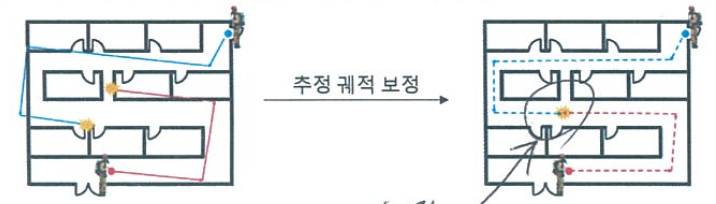
\includegraphics[width=.9\columnwidth]{figures/Section1/overview.png}
	\caption{이동궤적 오차 보정 연구 개요도}
	\label{fig:overview}
\end{figure}
\subsection{연구일정}
\lipsum[2]
\section{연구 내용}
\subsection{연구주제 1}
% Table example
\begin{table}[ht!]
    \centering
    \begin{tabular}{c c c c}
        \hline \hline
        $N$ & $J$ &  Algorithm & $\alpha$\\
        \hline
        3 & 0.6218 & sqp & 0.1\\
        4 & 0.5354 & sqp & 0.1\\
        5 & 0.4217 & sqp & 0.1\\
        \hline
        3 & 2.2954 & sqp & 0.9\\
        4 & 2.0849 & sqp & 0.9\\
        5 & 1.6180 & sqp & 0.9\\
        \hline \hline
    \end{tabular}
    \caption{Optimization result}
    \label{table:optimization_result}
\end{table}
\subsection{연구주제 2}
\subsection{연구주제 3}
% Cite example
\lipsum[3] \cite{lee2020vector}.
\section{결 론}
\lipsum[4]

% references
\bibliographystyle{unsrt}
\bibliography{references}

\end{document}
    